\def\title{Prueba}
\def\subtitle{Análisis crítico de información}
\def\curso{Probabilidad y estadística descriptiva e inferencial}

\documentclass{caes}

\begin{document}
%
\datos
%
\titulo{Objetivos de la evaluación}
\begin{itemize}[nosep]
    \item Representar datos gráficamente usando diagramas de caja.
    \item Argumentar y comunicar decisiones a partir del análisis crítico 
    de información presente en gráficas de carácter estadístico.
\end{itemize}

\titulo{Instrucciones generales}

\underline{La evaluación es individual y con nota al libro}, se puede usar
 calculadora pero no el celular. Además, para tener derecho a reclamo es 
 necesario contestar con lápiz pasta.

\titulo{Rubrica}

En la corrección, se le asignará puntaje a cada respuesta según los criterios 
que se encuentran detallados a continuación.

% {{\textbullet} Calcula correctamente la probabilidad acumulada de los datos.\\
%                     {\textbullet} Identifica correctamente las cinco partes que forman el 
%                     diagrama de caja.\\
%                     {\textbullet} Ubica correctamente el diagrama de caja en el plano.}

\begin{center}
\begin{tblr}{width=\linewidth, colspec={X[1]|X[5]}, hline{1,Z} = {1}{-}{}, hline{1,Z} = {2}{-}{}, hlines}
    Nivel de logro & \SetCell{c} Criterios o indicadores \\
    \SetCell[c=2]{c,black!15} Representación de datos (Ítem I.1) \\
    {Destacado\\ (5 puntos)} & 
    \begin{enu_tabla} 
        \item Calcula correctamente la probabilidad acumulada de los datos.
        \item Identifica correctamente las cinco partes que forman el diagrama de caja.
        \item Ubica correctamente el diagrama de caja en el plano.
    \end{enu_tabla} \\
    {Suficiente\\ (2 a 4 puntos)} & 
    \begin{enu_tabla}
        \item Tiene un error de arrastre en el cálculo de las probabilidades, pero muestra \mbox{dominio} del concepto.
        \item Identifica correctamente donde se abre y cierra la caja en el diagrama de caja.
        \item El diagrama representa a grandes rasgos la tendencia general de los datos.
    \end{enu_tabla}\\
    {Insuficiente\\ (0 o 1 punto)} & 
    \begin{enu_tabla}
        \item La metodología de cálculo es incorrecta y/o el diagrama caja no representa los datos entregados. 
    \end{enu_tabla}\\
    \SetCell[c=2]{c,black!15} Argumentación y comunicación de decisiones (Ítem I.2, II.1, II.2 y II.3) \\
    {Destacado\\ (5 puntos)} & 
    \begin{enu_tabla}
        \item Identifica correcta y completamente la información contenida en la gráfica.
        \item Argumenta utilizando evidencia estadística, para justificar la veracidad o falsedad de una conjetura, y evaluar el alcance y los límites de los argumentos utilizados. 
    \end{enu_tabla}\\
    {Suficiente\\ (2 a 4 puntos)} & 
    \begin{enu_tabla}
        \item La conclusión alcanzada es superficial y hace referencia solo a parte de los datos.
        \item Parte de los argumentos no se sustentan en la información entregada.
        \item No se refiere a la evidencia utilizando la terminología adecuada.
    \end{enu_tabla}\\
    {Insuficiente\\ (0 o 1 punto)} & 
    \begin{enu_tabla}
        \item No se logra extraer información y/o conclusiones significativas de la gráfica.
    \end{enu_tabla}\\

\end{tblr}    
\end{center}

\newpage

\parte El Instituto Nacional de Estadísticas (INE), realiza todos los años la 
Encuesta Suplemen\-taria de In\-gresos (ESI), para hacer catastro de la situación laboral
al interior de los hogares Chilenos. A con\-tinuación, se trabajará con una muestra de 
estos datos correspondiente al año 2020, para determinar si existe una diferencia 
salarial entre hombres y mujeres.

\pregunta La comparación de ingresos se realizará utilizando dos diagramas de cajas, uno para cada 
grupo. Su tarea es \underline{dibujar el diagrama de caja que representa los ingresos para las mujeres},
utilizando y com\-pletan\-do para este fin la tabla de datos que se encuentra a continuación. El diagrama para los 
hombres ya va incluido en la gráfica. 
%
\def\tablaA{%
\csvreader[
    tabularray = {
        cells = {c,m},
        vlines={wd=1pt},
        hlines={wd=1pt},
        hline{2} = {2}{-}{wd=1pt},
    }, 
    range = 1-13,
    table head = Sueldo (\$) & {Frecuencia\\ Acumulada} & {Probabilidad\\ Acumulada}\\,
]{sueldo_mujer_n28.csv}{1=\sueldo, 3=\cumN, 5=\cumP}%
{\sueldo & \cumN & }
}
\def\tablaB{%
\csvreader[
    tabularray = {
        cells = {c,m},
        vlines={wd=1pt},
        hlines={wd=1pt},
        hline{2} = {2}{-}{wd=1pt},
    }, 
    range = 14-25,
    table head = Sueldo (\$) & {Frecuencia\\ Acumulada} & {Probabilidad\\ Acumulada}\\,
]{sueldo_mujer_n28.csv}{1=\sueldo, 3=\cumN, 5=\cumP}%
{\sueldo & \cumN & }
}
%
\begin{center}
    \tikz \node (A) {\tablaA} node[right=1cm of A.north east, anchor=north west] {\tablaB};    
\end{center}
%
% # A tibble: 2 × 8
%    sexo     n     q1     q2     q3    iqr     low    high
%    <dbl> <int>  <dbl>  <dbl>  <dbl>  <dbl>   <dbl>   <dbl>
%    1(h)    32    318000 450592 555000 237000 -37500  910500 
%    2(m)    28    300395 380500 453062 152667  71394. 682062.

\begin{tcenter}
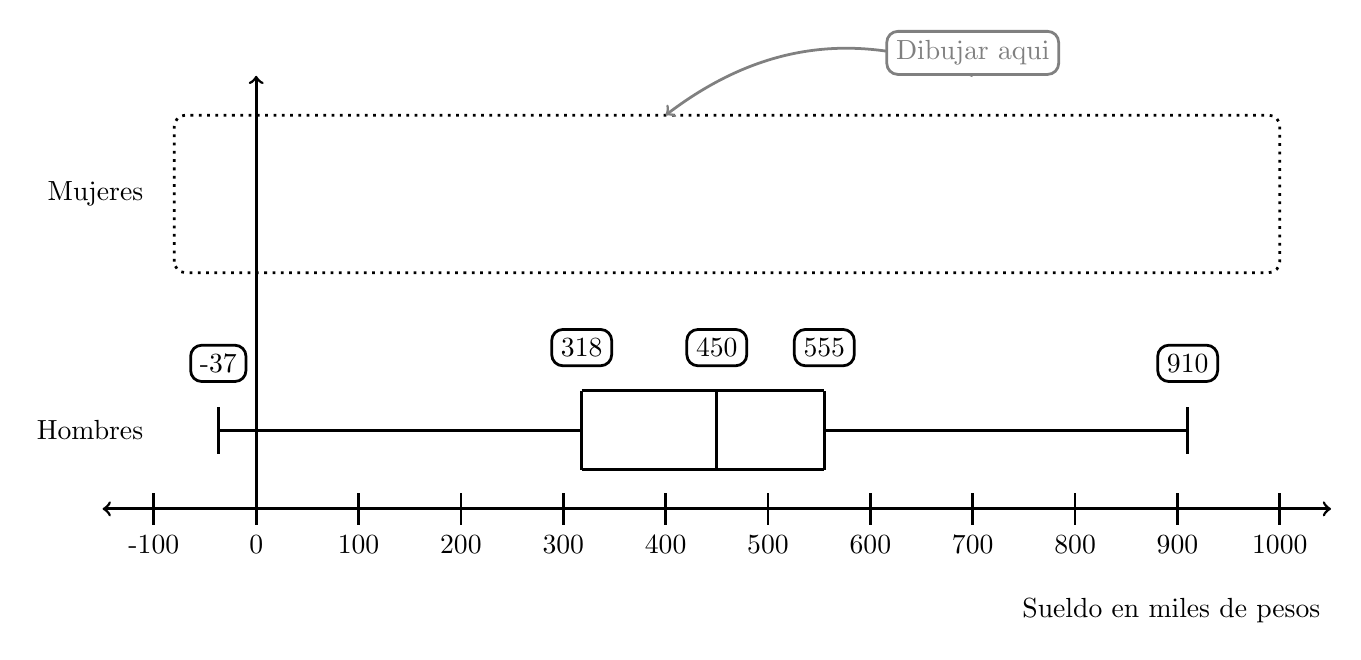
\begin{tikzpicture}[x=0.013cm,y=1cm,line width=1pt]
    \draw[<->] (-150,0) -- (1050,0) node[below=1cm,anchor=north east] {Sueldo en miles de pesos};
    \draw[->] (0,0) -- (0,5.5);
    %% boxplot hombres
    \foreach \x in {318,450,555} \draw (\x,0.5) -- (\x,1.5) node[above=3mm,draw,rounded corners] {\x};
    \foreach \x in {-37,910} \draw (\x,0.7) -- (\x,1.3) node[above=3mm,draw,rounded corners] {\x};
    \foreach \y in {0.5,1.5} \draw (318,\y) -- (555,\y);
    \draw (-37,1) -- (318,1);
    \draw (555,1) -- (910,1);
    %% draw y tikcs
    \node[left] at (-100,1) {Hombres};
    \node[left] at (-100,4) {Mujeres};
    %% draw x ticks
    \foreach \x in {-100,0,...,1000} \draw (\x,0.2) -- (\x,-0.2) node[below] {\x};
    %% instruction
    \draw[rounded corners, dotted] (-80,3) rectangle (1000,5);
    \draw[->,black!50] (700,5.5) node[above,draw,fill=white,rounded corners] {Dibujar aqui} to[bend right=30] (400, 5);
\end{tikzpicture}    
\end{tcenter}

\newpage 
\pregunta Basándose en la gráfica anterior, ¿Es posible decir que hay una brecha salarial
entre hombres y \mbox{mujeres} en Chile? ¿Si? ¿No? ¿Por qué? Desarrolle su respuesta.   
\respuesta[10]

\parte En esta sección se utilizarán los datos de la prueba SIMCE, correspondientes al 
año 2018, para estudiar el sistema educacional chileno. Para este fin, usted deberá 
interpretar las gráficas que se encuentran a continuación.

\begin{center}
    \includegraphics{/Users/fenho/Documents/r/simce_JS/grafico_prueba.pdf}    
\end{center}

\newpage
\pregunta ¿Qué información entrega \underline{la gráfica A}? ¿Qué conclusiones se pueden alcanzar 
a partir de esta gráfica? Desarrolle su respuesta y justifique. 
\respuesta[8]

\pregunta ¿Qué información entrega \underline{la gráfica B}? ¿Qué conclusiones se pueden alcanzar 
a partir de esta gráfica? Desarrolle su respuesta y justifique.
\respuesta[8]

\pregunta Considerando la información entregada \underline{por ambas gráficas juntas A y B}, 
¿A qué conclusiones se puede llegar con esta información? ¿Son distintas a las conclusiones 
alcanzadas anteriormente? Desarrolle su respuesta y justifique.
\respuesta[10]

\end{document}